\chapter{Daten und Zugrifsschichten}
\section{Einleitung}
Benutzer und App-Daten werden in zwei verschiedenen Datentöpfen gespeichert. Auf diese Datentöpfe soll nur durch Zugriffsschichten zugegriffen werden. Im Folgenden werden die Daten und die zugehörigen Zugrifsschichten genauer beschrieben.
\begin{figure}[htb]
    \centering
    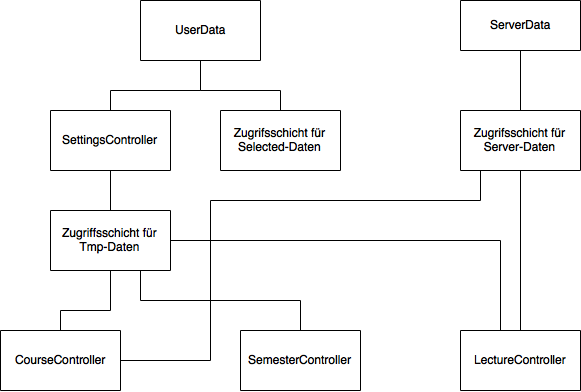
\includegraphics[width=\textwidth]{Daten}
    \caption{Daten und zugehörige Zugrifsschichten}
\end{figure}

Folgende Datentöpfe werden genutzt:
\begin{itemize}
     \item UserData
     \item ServerData
\end{itemize}

Folgende Zugrifssschichten sind vorhanden:
\begin{itemize}
     \item SelectedCourse
     \item SelectedSemester
     \item SelectedLectures
     \item AllChanges
     \item AllCourses
     \item AllLectures
\end{itemize}

\newpage
\chapter{Hintergrundaktualisierung}
\section{Einleitung}
Die App soll im Hintergrund regelmäßig prüfen ob neue Stundenplanänderungen für den Benutzer entstanden sind.
Daher wurde der Background Fetch implementiert.
\begin{figure}[htb]
    \centering
    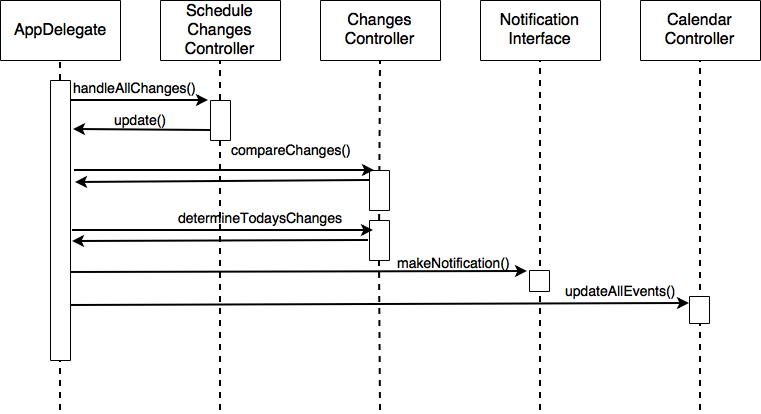
\includegraphics[width=\textwidth]{BackgroundFetch}
    \caption{Ablauf des Background Fetch}
\end{figure}

In diesem Sequenzdiagramm wird des Ablauf der application(performFetchWithCompletionHandler) Methode dargestellt. 
Zu Beginn werden durch den ScheduleChangesController die aktuellen Stundenplanänderungen vom Server geladen. 
Anschließend werden mit dem ChangesController die neu dazugekommenen Änderungen ermittelt und welche davon am aktuellen Tag stattfinden. Als Nächstes wird über das NotificationInterface eine lokale Notification für den User erstellt, die Ihn über die aktuellen Stundenplanänderungen informiert.
Zuletzt wird über den CalendarController der iOS Kalender aktualisiert.
\newpage
\section{CalendarController}
Der CalendarController ist der Controller für das Calendar Interface. Über ihn wird auf das Interface zugegriffen.

Im Folgenden wird auf die wichtigsten Methoden eingegangen:
\begin{itemize}
     \item createCalendar() -$>$ EKAuthorizationStatus
     \item removeCalendar()
     \item createAllEvents(lectures : [Lecture])
     \item updateAllEvents(changes : [ChangedLecture])
     \item removeAllEvents(lectures : [Lecture])
     \item CalendarRoutine() -$>$ Bool
\end{itemize}

Vor dem Ausführen der Aufgabe der jeweiligen Methode wird überprüft, ob der Benutzer die Berechtigung auf den Kalender zuzugreifen gewährt hat.

\subsection[createCalendar]{createCalendar() -$>$ EKAuthorizationStatus}
Erzeugt den Kalender falls die Berechtigung vorhanden ist. Falls er erzeugt wurde werden die Events mit createAllEvents in den Kalender geschrieben. Als Rückgabewert gibt er den Berechtigungsstatus zurück. Es gibt drei Rückgabewerte:
\begin{itemize}
     \item authorized \\[0.5em]
     Bedeutet, dass der Nutzer die Berechtigung erteilt hat und der Kalender angelegt wurde oder bereits angelegt war.
     \item notDetermined \\[0.5em]
     Bedeutet, dass die Berechtigung gerade abgefragt wird.
     \item denied \\[0.5em]
     Bedeutet, dass die Berechtigung verweigert wurden.
\end{itemize}

\subsection[removeCalendar]{removeCalendar()}
Löscht den Kalender und damit alle Einträge die darin vorhanden sind mit Hilfe des KalendarInterface.

\subsection[createAllEvents]{createAllEvents(lectures : [Lecture])}
Erzeugt aus den Vorlesungen die Events, die anschließend mit Hilfe des CalendarInterface in den Kalender geschrieben werden.
Falls der Kalender noch nicht erzeugt wurde, wird er angelegt.
Die EventID's werden mittels der saveIDs-Methode des CalendarInterface persistent gespeichert.

\subsection[updateAllEvents]{updateAllEvents(changes : [ChangedLecture])}
Ermittelt welche Art von Änderung vorliegt und passt mit Hilfe des CalendarInterface die  entsprechend Events im Kalender an.
Die EventID's werden mittels der saveIDs-Methode des CalendarInterface persistent gespeichert.

\subsection[removeAllEvents]{removeAllEvents(lectures : [Lecture])}
Holt sich für die übergebenden Vorlesungen die EventID's und löscht die entsprechenden Events mit Hilfe des CalendarInterface.
Die Änderungen an den EventID's werden mittels der saveIDs-Methode des CalendarInterface persistent gespeichert.

\subsection[CalendarRoutine]{CalendarRoutine() -$>$ Bool}
Aktualisiert die Vorlesungen im Kalender. Dazu holt sie sich die abgewählten und neu ausgewählten Vorlesungen und übergibt sie der removeAllEvents() oder createAllEvents()-Methode. Der Rückgabewert gibt an, ob der Benutzer die Berechtigung erteilt hat, in den Kalendar zu schreiben.

\newpage
\section{CalendarInterface}
Dies ist die Klasse die direkt auf den Kalender zugreift. 

Im Folgenden wird auf die wichtigsten Methoden eingegangen:
\begin{itemize}
     \item createCalenderIfNeeded() -$>$ Bool
     \item removeCalendar() -$>$ Bool
     \item createEvent(p\_event : EKEvent, key : String, isChanges : Bool)
     \item updateEvent(eventID : String, updatedEvent : EKEvent, key : String, lectureToChange : Bool)
     \item removeEvent(p\_eventId: String, p\_withNotes: Bool?=false) -$>$ Bool
     \item saveIDs()
\end{itemize}

\subsection[createCalenderIfNeeded]{createCalenderIfNeeded() -$>$ Bool}
Erzeugt den Kalender falls er nicht bereits vorhanden ist. Gibt einen Boolean-Wert zurück, ob der Kalender angelegt wurde.

\subsection[removeCalendar]{removeCalendar() -$>$ Bool}
Löscht den Kalender und damit alle Einträge, die er beinhaltet falls dieser vorhanden ist. Gibt einen Boolean-Wert zurück, ob das Löschen erfolgreich war.

\subsection[createEvent]{createEvent(p\_event : EKEvent, key : String, isChanges : Bool)}
Schreibt das übergebende Event in den Kalender. Unterscheidet dabei, ob es sich um eine Änderung oder eine normale Vorlesung handelt und fügt die EventID dem entsprechenden Dictonary hinzu. 

\subsection[updateEvent]{updateEvent(eventID : String, updatedEvent : EKEvent, key : String, lectureToChange : Bool)}
Das zu der EventID dazugehörige Event wird mit den entsprechend Werten des übergebenen Event angepasst. Durch den lectureToChange Boolean-Wert wird unterschieden, ob aus einer Vorlesung eine Änderung wird oder ob aus einer Änderung wieder eine Vorlesung wird. Dabei werden die EventsIDs in das entsprechende Dictonary verschoben.

\subsection[removeEvent]{removeEvent(p\_eventId: String, p\_withNotes: Bool?=false) -$>$ Bool}
Löscht das übergebene Event. Gibt einen Boolean-Wert zurück, ob das Löschen erfolgreich war.

\subsection[saveIDs]{saveIDs()}
Speichert die EventIDs der Vorlesungen und Änderungen in CalendarData persistent.

\newpage
\section{CalendarData}
Die CaledenarData-Klasse dient dazu, die EventIDs der Vorlesungen und Änderungen getrennt in Dictonarys zu speichern.
Die Dictonarys bestehen aus einer Zuordnung von einer ID einer Vorlesung zu mehreren EventIDs.

